\let\lesson\undefined
\newcommand{\lesson}{\phantomlesson{Bài tập vật lí nhiệt}}
\chapter[Bài tập vật lí nhiệt]{Bài tập vật lí nhiệt}
\section{Ôn tập lý thuyết}
\subsection{Khi nội năng của vật biến đổi chỉ bằng cách truyền nhiệt}
\begin{itemize}
	\item Nếu quá trình truyền nhiệt chỉ làm thay đổi nhiệt độ của vật, không làm vật chuyển thể thì:
	$$\Delta U=Q; \quad Q=mc\Delta t\quad \text{và}\quad Q_\text{thu}=Q_\text{toả}.$$
	\item Nếu quá trình truyền nhiệt làm vật chuyển từ thể này sang thể khác ở nhiệt độ không đổi thì:
	$$\Delta U=Q; \quad Q=\lambda m; Q=Lm \quad \text{và}\quad Q_\text{thu}=Q_\text{toả}.$$
\end{itemize}
\subsection{Khi nội năng của vật biến đổi bằng cả hai cách truyền nhiệt và thực hiện công}
$$\Delta U=Q+A$$
Các công thức tính công cơ học:
\begin{itemize}
	\item Công ngoại lực: $A=Fs\cos\alpha$;
	\item Công ngoại lực: $A=W_\text{đ2}-W_\text{đ1}$;
	\item Công ngoại lực:
	$A=\calP t$;
	\item Công lực thế: $A=W_\text{t1}-W_\text{t2}$.
\end{itemize}
\section{Mục tiêu cần đạt - Ví dụ minh hoạ}
\begin{dang}{Vận dụng định luật I nhiệt động lực học}
	\viduii{3}
	{Để làm nguội một sản phẩm bằng đồng có khối lượng $\SI{50}{\gram}$ đã bị nung nóng, người thợ thủ công thả nó vào một bình nhiệt lượng kế đựng $\SI{400}{\gram}$ nước ở $\SI{20}{\celsius}$ từ độ cao cách mặt nước trong bình $\SI{5}{\centi\meter}$. Khi sản phẩm đã nằm yên ở đáy bình và trong bình có cân bằng nhiệt thì nhiệt độ của nước là $\SI{22}{\celsius}$.
		\begin{enumerate}[label=\alph*)]
			\item Dựa vào cơ sở nào để biết nội năng của nước đã biến đổi? Tính độ biến thiên nội năng này.
			\item Nội năng của nước được biến đổi bằng những cách nào? Tính độ biến thiên nội năng của nước gây ra bởi mỗi cách.
			\item Sản phẩm được nung nóng tới nhiệt độ bao nhiêu?
		\end{enumerate}
	Biết độ cao của nước trong bình nhiệt lượng kế là $\SI{20}{\centi\meter}$, nhiệt dung riêng của nước là $\SI{4190}{\joule/\left(\kilogram\cdot\kelvin\right)}$, của đồng là $\SI{380}{\joule/\left(\kilogram\cdot\kelvin\right)}$; lấy $g=\SI{9.81}{\meter/\second^2}$. Bỏ qua sự truyền năng lượng của nước, sản phẩm cho bình nhiệt lượng kế và môi trường xung quanh. Coi lượng nước trong bình không đổi và lực đẩy Archimedes là không đáng kể.
}
{\hide{
Đây là bài toán về sự biến đổi nội năng bằng cả hai cách: nhận công và truyền nhiệt.\\
\textbf{	Xác định trạng thái ban đầu và cuối của hệ vật:}\\
 Vì bỏ qua mọi sự truyền năng lượng cho nhiệt lượng kế và môi trường xung quanh nên hệ trao đổi năng lượng chỉ có nước trong nhiệt lượng kế và sản phẩm.
	\begin{itemize}
		\item Trạng thái đầu: Nước ở nhiệt độ $t_1=\SI{20}{\celsius}$; sản phẩm ở độ cao $h_1=\SI{0.25}{\meter}$ so với đáy bình và nhiệt độ $\xsi{t}{\celsius}$.
		\item Trạng thái cuối: Nước ở nhiệt độ $t_2=\SI{22}{\celsius}$; sản phẩm ở độ cao $h_2=\SI{0}{\meter}$ và nhiệt độ $\SI{22}{\celsius}$.
	\end{itemize}
\begin{enumerate}[label=\alph*)]
	\item Dựa vào sự tăng nhiệt độ của nước mà biết nội năng của nước tăng.\\
	Do nước muốn tăng nhiệt độ $\Delta t_n=t_2-t_1$ thì phải nhận thêm nhiệt lượng $Q_n=m_nc_n\Delta t_n=\left(\SI{0.4}{\kilogram}\right)\cdot\left[\SI{4190}{\joule/\left(\kilogram\cdot\kelvin\right)}\right]\cdot\left(\SI{22}{\celsius}-\SI{20}{\celsius}\right)=\SI{3352}{\joule}$, nên độ tăng nội năng của nước là:
	$$\Delta U=Q_n=\SI{3352}{\joule}.$$
	\item Nội năng của nước tăng lên bằng hai cách là nhận công của sản phẩm khi rơi và nhận nhiệt của sản phẩm truyền cho.\\
	Sản phẩm rơi vào nước bị nước cản nên phải thực hiện công để chống lại sức cản của nước. Do bỏ qua tác dụng của lực đẩy Archimedes, nên công do sản phẩm thực hiện bằng công trọng lực của sản phẩm:
	$$A=W_\text{t1}-W_\text{t2}=mg\left(h_1-h_2\right)=\left(\SI{0.05}{\kilogram}\right)\cdot\left(\SI{9.81}{\meter/\second^2}\right)\cdot\left(\SI{0.25}{\meter}-\SI{0}{\meter}\right)\approx\SI{0.12}{\joule}.$$
	Độ tăng nội năng của nước do nhận được công là $\SI{0.12}{\joule}$.\\
	Sản phẩm bị nung nóng nên khi rơi vào nước nó truyền nhiệt cho nước. Theo định luật I nhiệt động lực học, ta tính được nhiệt lượng do sản phẩm toả ra:
	$$Q=\Delta U-A=\SI{3352}{\joule}-\SI{0.12}{\joule}=\SI{3351.88}{\joule}.$$
	Độ tăng nội năng của nước do truyền nhiệt là $\SI{3351.88}{\joule}.$
	\item Độ biến thiên nhiệt độ của sản phẩm:
	$$Q_s=m_sc_s\Delta t_s\Rightarrow \Delta t_s=\dfrac{Q_s}{m_sc_s}$$
	Vì nhiệt lượng do nước nhận được bằng nhiệt lượng do sản phẩm toả ra nên $Q_s=-Q=-\SI{3351.88}{\joule}.$
	\begin{eqnarray*}
	&	\Rightarrow& t_s-t_0=\dfrac{-\SI{3351.88}{\joule}}{\left(\SI{0.05}{\kilogram}\right)\cdot\left(\SI{380}{\joule/\kilogram\cdot\kelvin}\right)}\approx-\SI{176.41}{\celsius}
\\
&\Rightarrow& t_0=t_s+\SI{176.41}{\celsius}=\SI{198.41}{\celsius}.
	\end{eqnarray*}
\end{enumerate}}

}
	
\end{dang}
\begin{dang}{Bài toán về hiệu suất truyền nhiệt}
	\viduii{3}
	{Dùng bếp điện để đun một ấm nhôm khối lượng $\SI{600}{\gram}$ đựng 1,5 lít nước ở nhiệt độ $\SI{20}{\celsius}$. Sau 35 phút đã có $\SI{20}{\percent}$ lượng nước trong ấm hoá hơi ở nhiệt độ $\SI{100}{\celsius}$. Tính nhiệt lượng trung bình mà bếp điện cung cấp cho ấm nước trong mỗi giây, biết chỉ có $\SI{75}{\percent}$ nhiệt lượng mà bếp toả ra được dùng vào việc đun ấm nước. Biết nhiệt dung riêng của nhôm là $\SI{880}{\joule/\left(\kilogram\cdot\kelvin\right)}$, của nước là $\SI{4190}{\joule/\left(\kilogram\cdot\kelvin\right)}$; nhiệt hoá hơi riêng của nước ở nhiệt độ sôi $\SI{100}{\celsius}$ là $\SI{2.26E6}{\joule/\kilogram}$, khối lượng riêng của nước là $\SI{1}{\kilogram/\text{lít}}$.
}
{\hide{Gọi:
	\begin{itemize}
		\item $m_1$, $c_1$ lần lượt là khối lượng ấm nhôm và nhiệt dung riêng của nhôm;
		\item $m_2$, $c_2$ lần lượt là khối lượng của nước và nhiệt dung riêng của nước.
	\end{itemize}
	Khối lượng nước trong ấm:
	$$m_2=V_2D_2=\left(\SI{1.5}{\text{lít}}\right)\cdot\left(\SI{1.5}{\kilogram/\text{lít}}\right)=\SI{1.5}{\kilogram}.$$
	Nhiệt lượng ấm nhôm thu vào để tăng nhiệt độ từ $\SI{20}{\celsius}$ lên $\SI{100}{\celsius}$:
	$$Q_1=m_1c_1\Delta t=\left(\SI{0.6}{\kilogram}\right)\cdot\left[\SI{880}{\joule/\left(\kilogram\cdot\kelvin\right)}\right]\cdot\left(\SI{100}{\celsius}-\SI{20}{\celsius}\right)=\SI{42240}{\joule}.$$
	Nhiệt lượng nước thu vào để tăng nhiệt độ từ $\SI{20}{\celsius}$ lên $\SI{100}{\celsius}$ và $\SI{20}{\percent}$ lượng nước hoá thành hơi:
	$$Q_2=m_2c_2\Delta t+\SI{20}{\percent}m_2L=\left(\SI{1.5}{\kilogram}\right)\cdot\left[\SI{4190}{\joule/\left(\kilogram\cdot\kelvin\right)}\right]\cdot\left(\SI{80}{\celsius}\right)+\SI{20}{\percent}\cdot\left(\SI{1.5}{\kilogram}\right)\cdot\left(\SI{2.26E6}{\joule/\kilogram}\right)=\SI{1180.8}{\kilo\joule}.$$
	Nhiệt lượng do bếp điện cung cấp:
	$$Q=\dfrac{Q_1+Q_2}{H}=\SI{1630.72}{\kilo\joule}.$$
	Nhiệt lượng trung bình mà bếp điện cung cấp cho ấm nước trong mỗi giây:
	$$\calP=\dfrac{Q}{t}=\dfrac{\SI{1630.72}{\kilo\joule}}{35\cdot\SI{60}{\second}}\approx\SI{776.5}{\watt}.$$
}
}

\viduii{3}
{\begin{enumerate}[label=\alph*)]
		\item Tính nhiệt lượng cần thiết để $\SI{2}{\kilogram}$ nước đá ở $\SI{-10}{\celsius}$ hoá hơi hoàn toàn ở nhiệt độ sôi, cho biết:
		\begin{itemize}
			\item nhiệt dung riêng của nước đá là $\SI{1800}{\joule/\left(\kilogram\cdot\kelvin\right)}$;
			\item nhiệt dung riêng của nước $\SI{4200}{\joule/\left(\kilogram\cdot\kelvin\right)}$;
			\item nhiệt nóng chảy riêng của nước đá là $\SI{34E4}{\joule/\kilogram}$;
			\item nhiệt hoá hơi riêng của nước là $\SI{23E5}{\joule/\kilogram}$.
		\end{itemize}
	\item Nếu dùng một bếp dầu hoả có hiệu suất $\SI{80}{\percent}$, người ta phải đốt cháy hoàn toàn bao nhiêu lít dầu để cho $\SI{2}{\kilogram}$ nước đá ở $\SI{-10}{\celsius}$ biến thành hơi.\\
	Cho biết:
	\begin{itemize}
		\item khối lượng riêng của dầu hoả là $\SI{800}{\kilogram/\meter^3}$;
		\item năng suất toả nhiệt của dầu hoả là $\SI{44E6}{\joule/\kilogram}$.
	\end{itemize}
	\end{enumerate}

}
{\hide{\begin{enumerate}[label=\alph*)]
		\item Quá trình nước đá $\SI{-10}{\celsius}$ hoá hơi hoàn toàn ở nhiệt độ sôi trải qua 4 giai đoạn:
		\begin{itemize}
			\item Nước đá thu nhiệt để tăng nhiệt độ từ $\SI{-10}{\celsius}$ lên $\SI{0}{\celsius}$: 
			$$Q_1=mc_\text{đ}\left(0-t_0\right)=\left(\SI{2}{\kilogram}\right)\cdot\left[\SI{1800}{\joule/\left(\kilogram\cdot\kelvin\right)}\right]\cdot\left(\SI{10}{\celsius}\right)=\SI{36}{\kilo\joule}.$$
			\item Nước đá thu nhiệt để nóng chảy hoàn toàn ở $\SI{0}{\celsius}$:
			$$Q_2=m\lambda=\left(\SI{2}{\kilogram}\right)\cdot\left(\SI{34E4}{\joule/\kilogram}\right)=\SI{680}{\kilo\joule}.$$
			\item Nước thu nhiệt để tăng nhiệt độ từ $\SI{0}{\celsius}$ đến $\SI{100}{\celsius}$:
			$$Q_3=mc_\text{n}\left(\SI{100}{\celsius}-\SI{0}{\celsius}\right)=\left(\SI{2}{\kilogram}\right)\cdot\left[\SI{4200}{\joule/\left(\kilogram\cdot\kelvin\right)}\right]\cdot\left(\SI{100}{\celsius}\right)=\SI{840}{\kilo\joule}.$$
			\item Nước hoá hơi hoàn toàn ở $\SI{100}{\celsius}$:
			$$Q_4=mL=\left(\SI{2}{\kilogram}\right)\cdot\left(\SI{23E5}{\joule/\kilogram}\right)=\SI{4600}{\kilo\joule}.$$
		\end{itemize}
	Tổng nhiệt lượng đá cần thu vào để hoá hơi hoàn toàn ở $\SI{100}{\celsius}$:
	$$Q=Q_1+Q_2+Q_3+Q_4=\SI{6156}{\kilo\joule}.$$
	\item Nhiệt lượng bếp dầu cần cung cấp:
	$$Q_\text{tp}=\dfrac{Q}{H}=\dfrac{\SI{6156}{\kilo\joule}}{\SI{80}{\percent}}=\SI{7695}{\kilo\joule}.$$
	Khối lượng dầu cần đốt để tạo ra nhiệt lượng như trên:
	$$m=\dfrac{Q_\text{tp}}{q}=\dfrac{\SI{7695E3}{\joule}}{\SI{44E6}{\joule/\kilogram}}\approx\SI{0.175}{\kilogram}.$$
	Thể tích dầu cần đốt:
	$$V=\dfrac{m}{D}=\dfrac{\SI{0.175}{\kilogram}}{\SI{800}{\kilogram/\meter^3}}\approx\SI{2.19E-4}{\meter^3}=\SI{0.219}{\text{lít}}.$$
	\end{enumerate}
}
}
\end{dang}
\begin{dang}{Bài tập về động cơ nhiệt}
	\ppgiai{Động cơ nhiệt là thiết bị biến đổi nhiệt lượng thành công.\\
		\begin{itemize}
			\item \textbf{Nguyên tắc hoạt động của động cơ nhiệt}\\
			Tác nhân nhận nhiệt lượng $Q_1$ từ nguồn nóng biến một phần nhiệt lượng nhận được này thành công $A$ và toả phần nhiệt lượng $Q_2$ còn lại cho nguồn lạnh.
			\begin{center}
				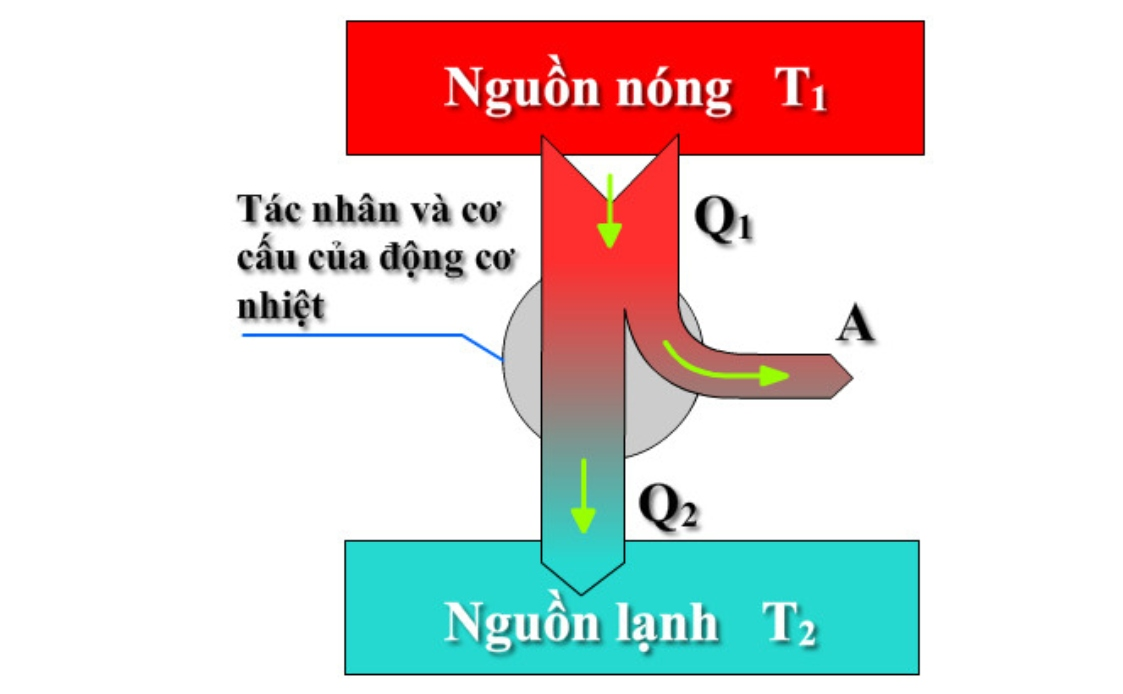
\includegraphics[width=0.55\linewidth]{../figs/VN12-Y24-PH-SYL-007-1}
			\end{center}
		\item \textbf{Hiệu suất của động cơ nhiệt}\\
		$$H=\dfrac{A}{Q_1}=\dfrac{Q_1-Q_2}{Q_1}=1-\dfrac{Q_2}{Q_1}.$$
		\luuy{Động cơ nhiệt không thể chuyển đổi toàn bộ nhiệt lượng nhận được thành công $\left(H<1\right)$.\\
		Hiệu suất cực đại của động cơ nhiệt:
	$$H_\text{max}=\dfrac{T_1-T_2}{T_1}.$$}
		\end{itemize}
	
}
\viduii{2}
{Một động cơ nhiệt làm việc sau một thời gian thì tác nhân đã nhận từ nguồn nóng nhiệt lượng $Q_1=\SI{1.5E6}{\joule}$, truyền cho nguồn lạnh nhiệt lượng $Q_2=\SI{1.2E6}{\joule}$. Hiệu suất thực của động cơ nhiệt này là bao nhiêu?

}
{\hide{
	Hiệu suất thực của động cơ nhiệt:
	$$H=1-\dfrac{Q_2}{Q_1}=1-\dfrac{\SI{1.2E6}{\joule}}{\SI{1.5E6}{\joule}}=\SI{20}{\percent}.$$
}
}
	\viduii{3}
	{Máy hơi nước công suất $\SI{10}{\kilo\watt}$ tiêu thụ $\SI{10}{\kilogram}$ than đá trong $\SI{1}{\text{giờ}}$. Biết hơi nước vào và ra cylanh có nhiệt độ $\SI{227}{\celsius}$ và $\SI{100}{\celsius}$. Năng suất toả nhiệt của than đá là $\SI{3.6E7}{\joule/\kilogram}$. Tính hiệu suất thực của máy và của một động cơ nhiệt lí tưởng làm việc với nhiệt độ nguồn nóng và nguồn lạnh nói trên.
	
}
{\hide{
	Hiệu suất của một động cơ nhiệt lí tưởng hoạt động giữa hai nguồn nhiệt $\SI{227}{\celsius}$ và $\SI{100}{\celsius}$:
	$$T_1=t_1+273=\SI{500}{\kelvin};\quad T_2=t_2+273=\SI{373}{\kelvin}.$$
	$$H_\text{max}=\dfrac{T_1-T_2}{T_1}=\SI{25.4}{\percent}.$$
	Hiệu suất thực của động cơ:
	$$H=\dfrac{A}{Q}=\dfrac{\calP t}{mq}=\dfrac{\left(\SI{10E3}{\watt}\right)\cdot\left(\SI{3600}{\second}\right)}{\left(\SI{10}{\kilogram}\right)\cdot\left(\SI{3.6E7}{\joule/\kilogram}\right)}=\SI{10}{\percent}.$$}
}
\end{dang}
